%!TEX root = ../main.tex
\chapter{Experimentos e Resultados}

Para comparar a qualidade e a performance da nossa solução com as abordagens anteriores, criamos três cenários de teste: (1) Prato de Cerâmica, (2) Caneca de Cerâmica, (3) Chave de Aço. Os parâmetros de materiais utilizados estão descritos na \tabref{tab:material_parameters}.

\begin{table}[ht]
\begin{center}
\begin{tabular}{c|ccccc}
Material & Densidade ($\nicefrac{kg}{m^3}$) & Módulo de Young (GPa) & Razão de Poisson & $\alpha$ & $\beta$\\
\hline Cerâmica & $2700$ & $7.4 \times 10^{10}$ & $0.19$ & $6$ & $1 \times 10^{-7}$\\
Aço & $1050$ & $3.5 \times 10^9$ & $0.34$ & $30$ & $8 \times 10^{-7}$\\
\end{tabular}
\end{center}
\caption{Parâmetros de Materiais}\label{tab:material_parameters}
\end{table}

Para cada cenário de teste, computamos os Coeficientes Multipolares usando a nossa abordagem e também computamos os Coeficientes Multipolares utilizando a abordagem descrita em \cite{zheng2010rigid}. Essa última que é a mesma utilizada em \cite{zheng2010rigid, zheng2011toward, langlois2014eigenmode}, utiliza o software comercial FastBEM \cite{fastbem}. Vale salientar que, para realizarmos a comparação, utilizamos a implementação original cedida pelos autores.

Os testes foram todos executados na mesma máquina. A \tabref{tab:benchmark_hardware} apresenta a especificação do Hardware utilizado.

\begin{table}[ht]
\begin{center}
\begin{tabular}{c|ccccc}
Componente & Especificação\\
\hline 
Placa-Mãe & SuperMicro X8DAH\\
CPU & Intel Xeon X5570 - 8-Core @2.93GHz\\
Memória RAM & 12x4GB DDR3 @1333MHz\\
GPU & GeForce TITAN BLACK 6GB DDR5
\end{tabular}
\end{center}
\caption{Especificações de Hardware}\label{tab:benchmark_hardware}
\end{table}

A \tabref{tab:benchmark_timings} apresenta a comparação de performance entre a nossa abordagem e as abordagens anteriores. A nossa abordagem obtem um speedup de mais de 30x em todos os cenários de teste.

\begin{table}[ht]
\begin{center}
\begin{tabular}{c|c|c c|c|c}
\multirow{2}{*}{Cenário}& \multirow{2}{*}{\# de modos} & \multicolumn{2}{c|}{Nosso Método} & FastBEM & \multirow{2}{*}{Speedup}\\
\cline{3-5}
& & Tempo (min) & Memória de GPU (MB) & Tempo (min)\\
\hline 
1 & 29 & 8.3 min & 578.1MB & 327.2 min & 39.42x\\
2 & 39 & 18.6 min & 998.7MB & 686.5 min & 36.90x\\
3 & 4 & 3.54 min & 1586.3MB & 102.9 min & 29.06x
\end{tabular}
\end{center}
\caption{Comparação de Performance entre a nossa solução e abordagens anteriores}\label{tab:benchmark_timings}
\end{table}

Também comparamos os valores numérico da nossa solução com os valores calculados pela abordagem anterior (Ver \figref{fig:coef_plate_delta}). A diferença numérica entre os métodos ficou abaixo de 5\%. Os demais gráficos e resultados numéricos estão disponíveis no Anexo A.

\begin{figure}[ht]
\centering
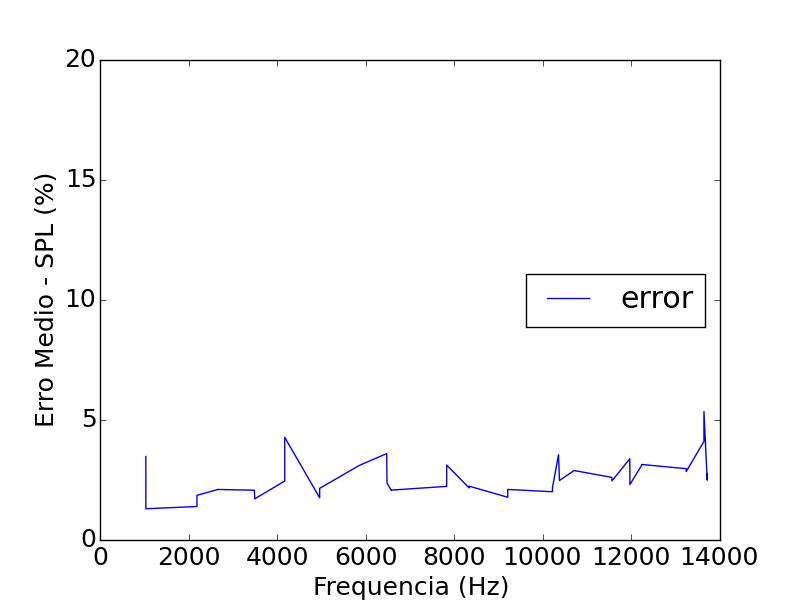
\includegraphics[width=0.6\textwidth]{../data/transfer_test/ceramic_plate/plots/ceramic_plate_error.png}
\caption[Comparação numérica para o Prato de Cerâmica]{Comparação numérica para o Prato de Cerâmica. O gráfico apresenta a diferença numérica média por frequência.}
\label{fig:coef_plate_delta}
\end{figure}

% \begin{figure}[ht] \label{fig:coef_mug_delta}
% \centering
% 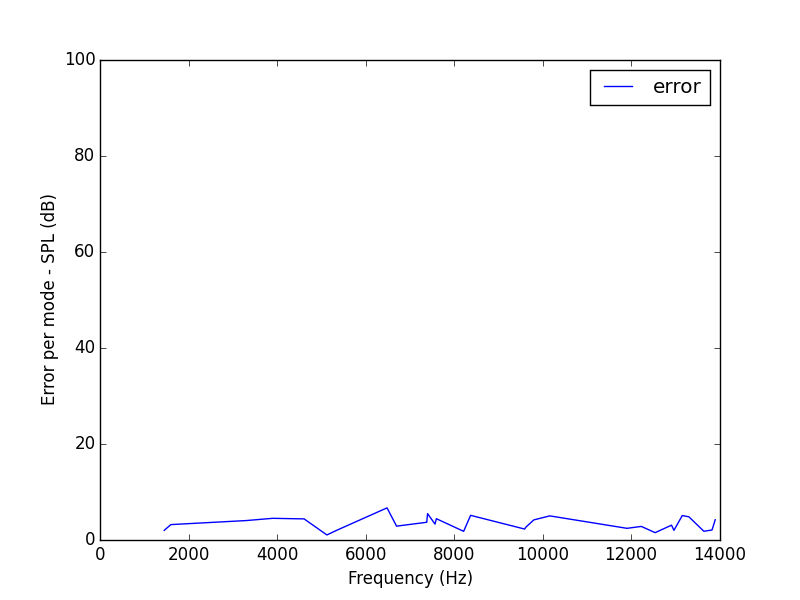
\includegraphics[width=0.6\textwidth]{../data/transfer_test/ceramic_mug/plots/ceramic_mug_error.png}
% \caption[Comparação numérica para a Caneca de Cerâmica]{Comparação numérica para a Caneca de Cerâmica. A figura ao topo apresenta o Erro Médio por frequência. As demais figuras apresentam a comparação para modos de vibração específicos.}
% \end{figure}

% \begin{figure}[ht] \label{fig:coef_key_delta}
% \centering
% 	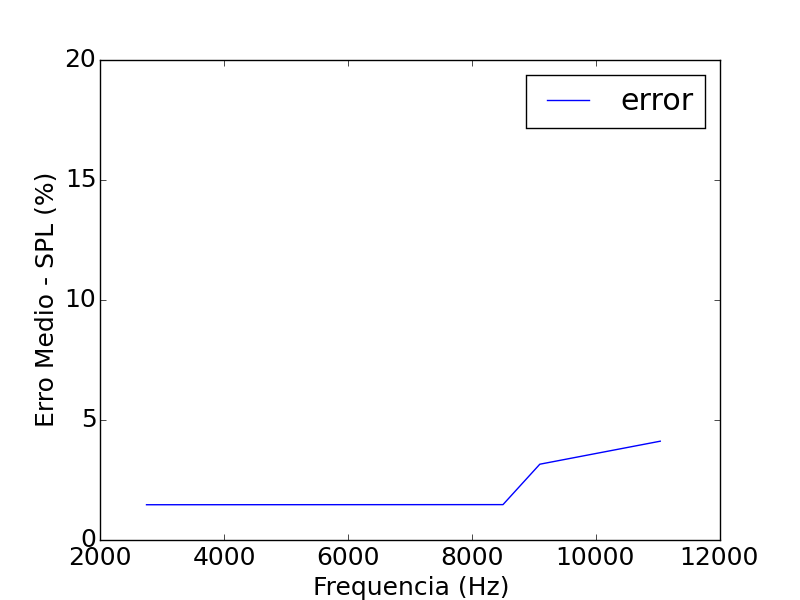
\includegraphics[width=0.6\textwidth]{../data/transfer_test/steel_key/plots/steel_key_error.png}
% \caption[Comparação numérica para a Chave de Aço]{Comparação numérica para a Chave de Aço. A figura ao topo apresenta o Erro Médio por frequência. As demais figuras apresentam a comparação para modos de vibração específicos.}
% \end{figure}

\section{Teste de Percepção}

Para testar a qualidade do áudio final, um teste A/B foi feito \footnote{A pesquisa está disponível em \url{https://docs.google.com/forms/d/1qfXssmKug0lh5uQXkot_XjWpjuSap4zJybzXG688XDY/viewform}}. Uma pesquisa foi feita utilizando a plataforma online Google Forms\cite{googleforms}. Nesse teste, o voluntário assistia uma série de pares de vídeos distintos. Enquanto a imagem dos vídeos de cada param era idêntica, o áudio de um deles foi gerado utilizando a abordagem anterior e o do outro foi gerado utilizando a nossa abordagem. Os vídeos de cada par eram identificados apenas por A ou B. O voluntário deveria responder à pergunta: ``Qual dos dois pareceu mais realista: A ou B?''. O voluntário tinha como opções: ``A'', ``B'' ou ``Não sei''.

A pesquisa foi divulgada em listas de e-mail de alunos e docentes de diferentes universidades e também em redes sociais. A \tabref{tab:survey_results} contém o resultado da pesquisa.

Em todos os testes, a maioria dos usuário considerou que o som gerado pelo nosso método era mais realista que ou tão realista quanto o som gerado pelos métodos anteriores. Considerando que o nosso objetivo era apenas acelerar o método, esses resultados excedem as nossas expectativas.

\begin{table}[ht]
\begin{center}
\begin{tabular}{c|ccccc}
Cena & Nosso Método & FastBEM & Não sei & Total\\
\hline Prato de Cerâmica & $70.5\%$ & $24\%$ & $5.5\%$ & $100\%$\\
Caneca de Cerâmica & $64.6\%$ & $24\%$ & $11.4\%$ & $100\%$\\
Prato de Cerâmica & $46.9\%$ & $20.5\%$ & $32.7\%$ & $100\%$\\
Total & & & & 254 respostas
\end{tabular}
\end{center}
\caption{Resultado dos Testes de Percepção}\label{tab:survey_results}
\end{table}




